\documentclass{article}
\usepackage[portuguese]{babel}
\usepackage[utf8]{inputenc}
\usepackage[margin=1in]{geometry}
\usepackage{graphicx}
\usepackage{biblatex}
\usepackage{csquotes}
\usepackage{float}
\usepackage{titlesec}
\usepackage{array}
\usepackage{tabularx}
\usepackage{hyperref}
\usepackage{fancyhdr}
\usepackage{listings}
\hypersetup{
    colorlinks,
    citecolor=black,
    filecolor=black,
    linkcolor=black,
    urlcolor=black
}
\lstset{
  language=C,                % choose the language of the code
  %numbers=left,                   % where to put the line-numbers
  stepnumber=1,                   % the step between two line-numbers.        
  numbersep=5pt,                  % how far the line-numbers are from the code
  backgroundcolor=\color{white},  % choose the background color. You must add \usepackage{color}
  showspaces=false,               % show spaces adding particular underscores
  showstringspaces=false,         % underline spaces within strings
  showtabs=false,                 % show tabs within strings adding particular underscores
  tabsize=2,                      % sets default tabsize to 2 spaces
  captionpos=b,                   % sets the caption-position to bottom
  breaklines=true,                % sets automatic line breaking
  breakatwhitespace=true,         % sets if automatic breaks should only happen at whitespace
  title=\lstname,                 % show the filename of files included with \lstinputlisting;
}

\setlength{\parindent}{4em}
\setlength{\parskip}{1em}
\renewcommand{\baselinestretch}{1.5}

\pagestyle{fancy}
\fancyfoot{}
\fancyfoot[R]{\thepage}
\addbibresource{references.bib}

\begin{document}
\nocite{geeksMemoryAllocation}
\nocite{pointerMedium}
\nocite{cDataType}
\nocite{staticAndDynamicAllocation}
\nocite{memoryAllocation}

\thispagestyle{empty}

\noindent\begin{minipage}{0.3\textwidth}
    
\includegraphics[scale=0.15]{assets/logo-unicamp.pdf}
\end{minipage}
\hfill
\begin{minipage}{0.6\textwidth}\raggedleft
    UNIVERSIDADE ESTADUAL DE CAMPINAS

    FACULDADE DE TECNOLOGIA DA UNICAMP
    
    SI201 B - Monitoria
    
    Izael Souza
\end{minipage}
\begin{center}
    \hfill%
\end{center}

\begin{center}
    \textbf{\huge Alocação de Memória e Ponteiros}
    
\end{center}

\vspace*{\fill}
\begin{center}
    \textbf{Limeira, SP - Brasil}
    
    \textbf{Junho 2021}
\end{center}

\thispagestyle{empty}
\renewcommand* \contentsname{Sumário}
\tableofcontents

\section{Introdução a Memória em C}

\subsection{Layout de Memória em C}

Uma representação típica de memória de um programa em C consiste das seguintes partes:
\begin{itemize}
  \item \textbf{Segmento de texto:} seções de um programa que contém instruções de execução;
  \item \textbf{Segmento de dados inicializados:} porção do espaço de endereço virtual que contém
    variáveis globais e estáticas que foram inicializadas pelo programador;
  \item \textbf{Segmento de dados não inicializados (BSS):} aqui ficam as variáveis globais e
    estáticas não inicializados pelo programador ou inicializados com valor 0;
  \item \textbf{\textit{Heap}}: onde acontece a \textbf{alocação dinâmica}. Ela começa no final do segmento BSS e vai
    crescendo de tamanho. Ela é gerenciada por \textbf{\textit{malloc()}}, \textbf{\textit{realloc()}} e \textbf{\textit{free()}};
  \item \textbf{\textit{Stack}}: onde fica a \textbf{\textit{stack}} do programa, com política LIFO (\textit{Last In First
    Out}).Variáveis automáticas são armazenadas aqui e informações salvas a cada chamada de uma
    função. Essa parte da memória é vital para o funcionamento de recursões em C;
\end{itemize}

\begin{figure}[H]
  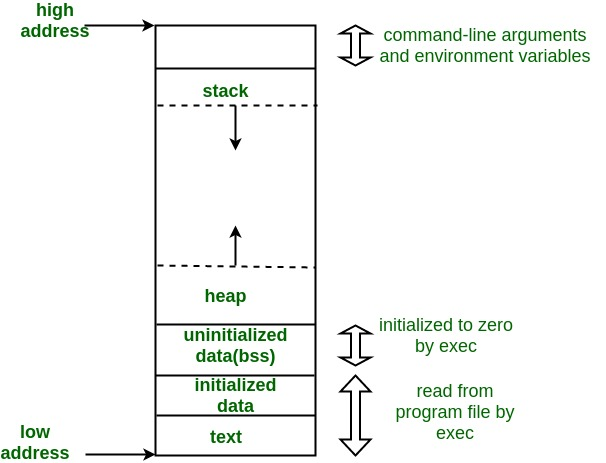
\includegraphics[scale=0.5]{assets/memory-layout-c.jpeg}
  \centering
  \caption{Layout de memória de programas em C - GeeksforGeeks}
\end{figure}

\subsection{\textit{Heap} e \textit{Stack}}

\paragraph{Heap} Na Heap, a memória é alocada durante a execução das instruções (código) escrito.
Ela é um espaço de memória disponível para desenvolvedores manipulá-la, alocando e desacolando
blocos de memória conforme necessário. Quando fazemos um objeto ele é criado na Heap e as
informações de referência são sempre armazenadas na \textbf{\textit{Stack}}. Um ponto importante quando
estamos manipulando a Heap é tomar cuidado para não termos um vazamento de memória (\textit{Memory
Leak}). Por isso é importante estarmos usando a função \textbf{\textit{free()}}.

\paragraph{Stack} Na Stack, a alocação acontece em blocos de memória contíguos. Aqui, o tamanho de
memória a ser alocada é conhecida pelo compilador e, sempre que uma função é chamada, suas variáveis
tem sua memória alocada na \textbf{\textit{Stack}}. Um ponto a ressaltar aqui é que o programador não precisa
se preocupar em ficar alocando e desalocando memória explicitamente, já que todo esse processo é
responsabilidade do compilador.
\subsection{Variáveis em C}

Antes de entender como os ponteiros funcionam precisamos relembrar o conceito de variável.
Uma variável é um bloco reservado na memória para armazenar algum valor. Em C podemos definir e inicializar
uma variável da seguinte forma:

\begin{lstlisting}[language=C]
int x = 0;
\end{lstlisting}

O primeiro termo se refere ao \textit{datatype} da variável, o segundo termo se refere ao nome daquela
variável que vamos usar para acessá-la e o terceiro termo é o valor que vamos armazenar naquele bloco. Além disso, podemos acessar também o endereço de memória onde
aquele bloco foi reservado.

\begin{lstlisting}[language=C]
int x = 0;
printf("O endereco e: %d", &x);
\end{lstlisting}

O código de bloco acima realiza \textbf{alocação de memória estática}, ou seja, a alocação da memória
é feita pelo compilador e não podemos mudar seu tamanho depois de alocada.

Devemos lembrar que cada tipo de variável ocupa um espaço na memória. Por exemplo, uma variável
do tipo \textbf{\textit{int}} ocupa 4 \textit{bytes}. Já uma variável do tipo \textbf{\textit{long long int}} ocupa 8 \textit{bytes}.
Saber disso é importante para garantirmos que não estamos desperdiçando espaço ou que temos espaço suficiente
para o que desejamos, e será algo que vamos precisar quando formos realizar alocação dinâmica.

\subsection{Definição e Notação de Ponteiros}
Quando digitamos \textbf{\textit{int x = 0;}} estamos armazenando o valor 0 na variável \textbf{\textit{x}}. No entanto,
também podemos armazenar o \textbf{endereço} de cada variável em uma outra variável de um tipo específico:
\textbf{variável ponteiro}.

\begin{lstlisting}[language=C]
int x = 0;
int* ptrX = &x;
printf("O valor e: %d", x);
printf("O endereco e: %d", ptrX);
\end{lstlisting}

Note que temos o \textbf{\textit{*}} logo depois do \textbf{\textit{int}}. Ele nos diz que o tipo daquela variável é um
ponteiro para um \textbf{\textit{int}}, ou seja, ela não armazena um \textbf{\textit{int}} propriamente dito, mas sim o
endereço de uma variável do tipo \textbf{\textit{int}}.

Além disso, note que usamos o \textbf{\textit{\%d}} para estarmos mostrando o endereço que aquele
ponteiro está armazenando. Isso não é totalmente correto, pois endereços de memórias devem ser mostrados
como hexadecimais. Dessa forma o mais correto seria usar o \textbf{\textit{\%p}} para mostrar ponteiros. No entanto,
endereços de memória também pode ser mostrando com um inteiro decimal ou como octais,
por isso o código anterior não acusa nenhum erro.


\section{Alocação de Memória Dinâmica}
Nós comentamos um pouco na primeira seção sobre alocação estática de memória. Agora vamos comentar sobre
\textbf{Alocação Dinâmica de Memória}. Nesse caso, a alocação ocorre durante o \textit{runtime} do programa.
Mas, porque precisamos disso? Alocação de memória durante o tempo de execução do programa nos permite uma maior
flexibilidade com a memória, ou seja, conseguimos gerenciar a memória que precisamos, sem alocar mais
ou menos que o necessário. Na maioria das vezes, vamos usar alocação dinâmica para tipos de dados
derivados, ou seja, \textbf{\textit{pointer types}}, \textbf{\textit{array}}, \textbf{\textit{structures}} (registros), etc.

\subsection{Como alocar dinamicamente?}
As 4 funções em C referente a alocação dinâmica de memória estão definidas na \textit{stdlib.h}, sendo elas:
\begin{itemize}
  \item \textit{\textbf{malloc()} \footnote{Mais comum quando trabalhamos com alocação dinâmica.}}: abreviação para \textit{memory allocation}. Essa função reserva um bloco de memória
    com o tamanho especificado de \textit{bytes}, e retorna um \textbf{ponteiro} do tipo \textbf{\textit{void}}
    que podemos dar \textit{cast} para outro tipo de dado. 
  \item \textbf{\textit{realloc()}}: caso a memória previamente alocada dinamicamente for insuficiente (ou maior do que necessário)
    podemos mudar o tamanho dela usando a função \textbf{\textit{realloc}}, especificando o novo tamanho da memória.
  \item \textbf{\textit{calloc()}}: abreviação para \textit{contiguous allocation}. A diferença entre \textbf{\textit{malloc}} e \textbf{\textit{calloc}}
    é que o segundo aloca a memória e inicializa todos os \textit{bits} para zero.
  \item \textbf{\textit{free()}}: memória dinamicamente alocada não são liberadas sozinhas, já que as mesma
    estão sendo alocadas na Heap. Dessa forma, precisamos explicitamente liberar elas usando a função \textbf{\textit{free()}}.
    Caso não liberamos a memória, pode ocorrer o \textbf{\textit{Memory Leak}}, reduzindo a performance e a
    quantidade de memória disponível.
\end{itemize}

\subsection{Sintaxe das Funções}
\begin{lstlisting}[language=C]
ptr = (castType*)malloc(size)
ptr = (castType*)calloc(n, size)
ptr = realloc(ptr, x)
free(ptr)
\end{lstlisting}

\subsection{Exemplo de Uso - \textit{malloc()}}
Fazemos parte de uma universidade e precisamos guardar alguns dados dos alunos:
\begin{itemize}
    \item Nome Completo;
    \item Data de Nascimento;
    \item RA;
    \item Quantidade de matérias cursadas;
    \item Matérias cursadas;
    \item Data limite para Integralização;
\end{itemize}

Todos os dados mencionados acima serão do tipo \textbf{\textit{string}} ou um \textbf{\textit{array}} de \textbf{\textit{strings}}. Sabendo disso, como podemos abordar esse problema?

\subsubsection{Criando a Estrutura Aluno}
Como estamos na linguagem C, podemos usar uma \textbf{\textit{struct} Aluno} a qual é composta pelos dados acima. Dessa forma, teremos:
\begin{lstlisting}[language=C]
typedef struct Aluno {
    char *nomeCompleto;
    char *dataDeNascimento;
    char *ra;
    char **materiasCursadas;
    char *limiteIntegralizacao;
    int qtdMaterias;
} Aluno;
\end{lstlisting}

\subsubsection{Função para Criar um Novo Aluno}
Até momento apenas definimos a estrutura aluno. Não podemos de fato usar ainda. Lembre-se, aqui estamos tratando de uma \textbf{\textit{struct}}, logo temos que alocar espaço na memória para estarmos manipulando a mesma. Para isso, podemos fazer uma função \textbf{newAluno()}, que recebem alguns parâmetros e retorna um \textbf{ponteiro} para a \textbf{\textit{struct}} do tipo \textbf{\textit{Aluno}}:
\begin{lstlisting}[language=C]
Aluno *newAluno(char *nomeCompleto, char *dataDeNascimento, char *ra, char *limiteIntegralizacao)
{
    Aluno *aux = (Aluno *)malloc(sizeof(Aluno);
    aux->nomeCompleto = nomeCompleto;
    aux->dataDeNascimento = dataDeNascimento;
    aux->ra = ra;
    aux->materiasCursadas = (char **)malloc(sizeof(char *) * 7);
    aux->limiteIntegralizacao = limiteIntegralizacao;
    aux->qtdMaterias = 0;
    return aux;
}
\end{lstlisting}

Note que para as materias cursadas, tivemos um \textbf{\textit{cast}} para ponteiro de ponteiro de \textbf{\textit{char}} e no \textbf{\textit{malloc()}}, usamos o \textbf{\textit{sizeof(char *)}} a multiplicamos esse valor por 7 \footnote{O valor 7 foi escolhido aleatoriamente. Podemos colocar qualquer valor aqui.}, assim podemos ter 7 registros. Percebe um padrão? Apenas removemos um '*'. No caso de \textbf{\textit{char ***}}, teríamos \textbf{\textit{sizeof(char **)}}.

\subsubsection{Adicionando Matérias}
Agora, temos que pensar em como podemos adicionar matérias. No nosso caso, \textbf{\textit{materiasCursadas}} é um \textbf{\textit{char **}}, ou seja, ponteiro de ponteiro. Dessa forma, temos um \textbf{\textit{array}} de \textbf{\textit{strings}}. Sabendo disso, podemos criar uma função \textbf{\textit{addMaterial()}}, que recebe como parâmetro um ponteiro para Aluno, e um \textbf{\textit{string}} matéria:
\begin{lstlisting}[language=C]
void addMaterial(Aluno *aluno, char *materia)
{
    printf("Adicionando a materia: %s\n", materia);
    aluno->materiasCursadas[aluno->qtdMaterias++] = materia;
}
\end{lstlisting}

No bloco de código acima, estamos pegando o vetor \textbf{\textit{materiasCursadas}} e, baseando na quantidade de matérias que temos (inicialmente 0), estamos adicionando uma nova matéria e, em seguida, temos que somar 1 à \textbf{\textit{qtdMateria}}, já que uma nova matéria foi adicionada.

\subsubsection{Usando Aluno}
Agora que temos as principais parte do código prontas, podemos estar usand-o. Primeiramente, vamos criar um novo aluno passando alguns argumentos para ele e, em seguida, vamos adicionar algumas matérias:
\begin{lstlisting}[language=C]
int main()
{
    // Criando o aluno "Miguel"
    Aluno *aluno = newAluno("Miguel", "24/05/2000", "567784", "31/12/2027");
    
    // Adicionando materias para Miguel
    addMateria(aluno, "SI201");
    addMateria(aluno, "SI401");
    addMateria(aluno, "TT002");
    addMateria(aluno, "ST562");
    
    // Printando materias de Miguel
    for(int i = 0; i < aluno->qtdMaterias; i++)
    {
        printf("%s\n", aluno->materiasCursadas[i]);
    }

    return 0;
}
\end{lstlisting}

\subsubsection{Pontos Importantes}
Apesar do código acima estar funcional, tem algumas coisas que podemos melhorar:
\begin{itemize}
    \item Podemos criar uma função para printarmos as informações dos alunos;
    \item Quando alocamos \textbf{\textit{materiasCursadas}}, pegamos o tamanhao de \textbf{\textit{char *}} e multiplicamos por 7, ou seja, podemos ter 7 entradas dentro desse nosso \textbf{\textit{array}}. O que acontece se tivermos mais? E se tivermos menos? Como podemos estar contornando isso? (Dica: função relacionada a alocação dinâmica);
    \item Como podemos fazer para excluirmos uma matéria?
\end{itemize}
\addtocontents{toc}{\protect\thispagestyle{empty}}
\pagenumbering{gobble}
\fancyhead{}
\printbibliography[heading=bibintoc, title={Referências}]


\end{document}

